\documentclass[12pt, a4paper]{article}

% Lingua e codifica
\usepackage[utf8]{inputenc}
\usepackage[italian]{babel}
\usepackage[T1]{fontenc}

% Matematica
\usepackage{amsmath, amsfonts, amssymb}

% Immagini
\usepackage{graphicx}
\graphicspath{{./images/}}

% Margini
\usepackage[margin=2.5cm]{geometry}
\setlength{\headheight}{14.5pt}
\addtolength{\topmargin}{-2.5pt}

% Colori
\usepackage[dvipsnames]{xcolor}

% Tabelle e figure
\usepackage{booktabs}
\usepackage{caption}
\usepackage{subcaption}
\usepackage{float}

% Spaziatura paragrafi
\usepackage{parskip}
\setlength{\parindent}{0pt}

% Collegamenti ipertestuali
\usepackage{hyperref}
\hypersetup{
    colorlinks=true,
    linkcolor=blue,
    filecolor=magenta,
    urlcolor=cyan,
    pdftitle={Domande Bio},
    pdfauthor={Matias Bonoli},
}

% ─── Comando domanda (1, 2, 3, ...) compare nell'indice ────────────────────

\title{\textbf{Domande Bio}}
\author{Matias Bonoli}
\date{\today}

% ─────────────────────────────────────────────────────────────────────────────
\begin{document}

\maketitle
\tableofcontents
\newpage

\section{Si spieghi come possiamo calcolare la distanza di edit tra due stringhe v e w utilizzando la griglia dove gli archi sono pesati. Come si ricostruisce una matrice di allineamento che riflette la distanza di edit?}

La \textbf{distanza di edit} è definita come il numero minimo di operazioni elementari (delezione, inserzione, sostituzione) necessarie per trasformare una stringa nell'altra.
\begin{equation}
    d_E(v, w) = \text{MIN numero di operazioni per trasformare } v \text{ in } w
\end{equation}

\textbf{Esempio di trasformazione}

\textbf{TGCATAT} $\rightarrow$ \textbf{ATCCGAT} in 4 passi:
\begin{itemize}
  \item TGCATAT \quad $\rightarrow$ (inserisco \textcolor{blue}{A} all'inizio)
  \item \textcolor{blue}{A}TGCATAT \quad $\rightarrow$ (sostituisco \textcolor{red}{C} al posto della 3$^\circ$ \textcolor{red}{G})
  \item AT\textcolor{red}{C}CATAT \quad $\rightarrow$ (sostituisco \textcolor{red}{G} al posto della 5$^\circ$ \textcolor{red}{A})
  \item ATCC\textcolor{red}{G}TAT \quad $\rightarrow$ (cancello la 6$^\circ$ \textcolor{cyan}{T})
  \item ATCCG\textcolor{cyan}{A}T \quad (fatto)
\end{itemize}

Per calcolare la distanza di edit $d_E(v, w)$ in modo efficiente si costruisce una \textbf{griglia di edit} (alignment grid) con archi pesati e si applica la \textbf{programmazione dinamica}.

Date due stringhe $v$ e $w$, con $n=|v|$ e $m=|w|$ la \textbf{griglia di edit} è un grafo orientato $G=(V, E)$ di dimensioni 
$(n+1) \times (m+1)$, i cui vertici sono coppie $(i, j)$ con $0 \leq i \leq n$ e $0 \leq j \leq m$.
Ogni vertice, inoltre, rappresenta l'allineamento tra prefissi $v[1..i]$ e $w[1..j]$. 
Il vertice $(0,0)$ è il \textbf{nodo sorgente} mentre $(n,m)$ è lo \textbf{stato finale} (sink).
Gli archi della griglia sono i movimenti permessi sulla griglia e sono etichettati mediante \textbf{funzione di costo}.
Ogni cammino da $(0,0)$ a $(n,m)$ rapprensenta un possibile allineamento fra $v$ e $w$, mentre il costo complessivo rappresenta il costo dell'allineamento.
Ogni cammino valido nella griglia da sorgente a sink corrisponde esattamente a un allineamento tra $v$ e $w$. Il costo del cammino (somma dei pesi degli archi) è il numero di operazioni di editing.

I movimenti permessi e i loro pesi (costi) sono:
\begin{itemize}
    \item \textbf{Spostamento verticale} da $(i-1, j)$ a $(i, j)$: corrisponde all'inserimento di un gap (\texttt{-}) nella stringa $w$ (delezione di $v_i$). 
    \item \textbf{Spostamento orizzontale} da $(i, j-1)$ a $(i, j)$: corrisponde all'inserimento di un gap (\texttt{-}) nella stringa $v$ (inserimento di $w_j$).
    \item \textbf{Spostamento diagonale} da $(i-1, j-1)$ a $(i, j)$: corrisponde all'allineamento di $v_i$ con $w_j$. (\textit{match} se $v_i = w_j$, \textit{sostituzione} se $v_i \neq w_j$).
\end{itemize}

Formalmente, la \textbf{funzione di costo} $\delta$ assegna un costo alla coppia di simboli che vengono allineati:
\begin{itemize}
    \item \textbf{Match} (caratteri identici): $\delta(v_i,w_j)=0$ se $v_i = w_j$ (ad esempio $\delta(A,A)=0$), poiché non è richiesta alcuna operazione di modifica.
    \item \textbf{Mismatch} (sostituzione): $\delta(v_i,w_j)=1$ se $v_i \neq w_j$ (ad esempio $\delta(A,C)=1$).
    \item \textbf{Indel} (inserzione o delezione): $\delta(v_i,\text{-})=1$ per una delezione e $\delta(\text{-},w_j)=1$ per una inserzione.
\end{itemize}

Questi costi diventano i pesi degli archi nella griglia di edit:
\begin{itemize}
    \item l'arco verticale da $(i-1,j)$ a $(i,j)$ ha peso $\delta(v_i,\text{-})=1$;
    \item l'arco orizzontale da $(i,j-1)$ a $(i,j)$ ha peso $\delta(\text{-},w_j)=1$;
    \item l'arco diagonale da $(i-1,j-1)$ a $(i,j)$ ha peso $\delta(v_i,w_j)$, quindi $0$ se $v_i = w_j$ e $1$ se $v_i \neq w_j$.
\end{itemize}

\begin{figure}[h]
    \centering
    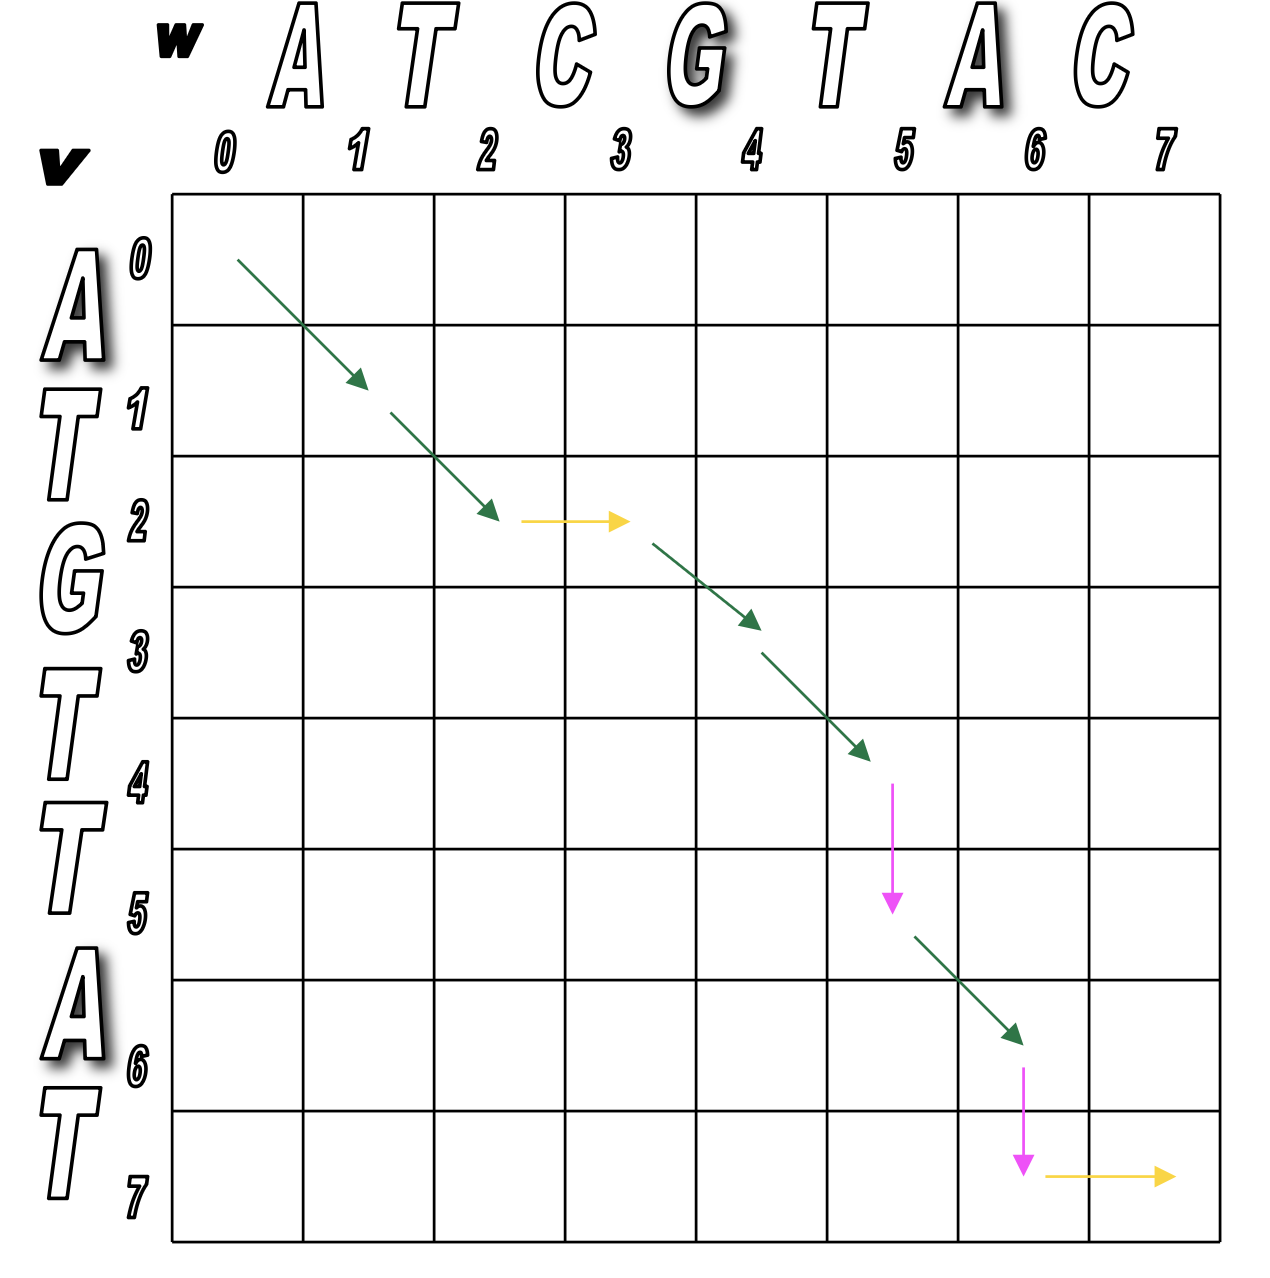
\includegraphics[width=0.7\textwidth]{images/edit_graph.png}
    \caption{Didascalia dell'immagine}
    \label{fig:edit grid}
\end{figure}

Per calcolare il costo minimo per raggiungere un nodo $(i,j)$ si applica la programmazione dinamica. Prima si definiscono i \textbf{casi base} (inizializzazione della prima riga e prima colonna):
\begin{itemize}
    \item $S(i, 0) = i$ per $0 \leq i \leq n$
    \item $S(0, j) = j$ per $0 \leq j \leq m$
\end{itemize}

Successivamente, si riempie il resto della griglia con la seguente \textbf{equazione di ricorrenza}:
\begin{equation}
    S(i, j) = \min
    \begin{cases}
        S(i-1, j) + 1 & \text{(Delezione)} \\
        S(i, j-1) + 1 & \text{(Inserzione)} \\
        S(i-1, j-1) + \delta(v_i, w_j) & \text{(Match/Mismatch)}
    \end{cases}
\end{equation}
dove $\delta(v_i, w_j) = 0$ se $v_i = w_j$, e $1$ altrimenti.
Il valore calcolato nel nodo \textit{sink}, ovvero $S(n, m)$, rappresenta la \textbf{distanza di edit ottima}. La \textbf{complessità} di calcolo, dovendo valutare un'operazione costante per ogni cella della griglia, è di $\mathcal{O}(n \times m)$ in tempo e in spazio.

\vspace{0.5cm}
\textbf{Ricostruzione della matrice di allineamento}

\begin{figure}[h]
    \centering
    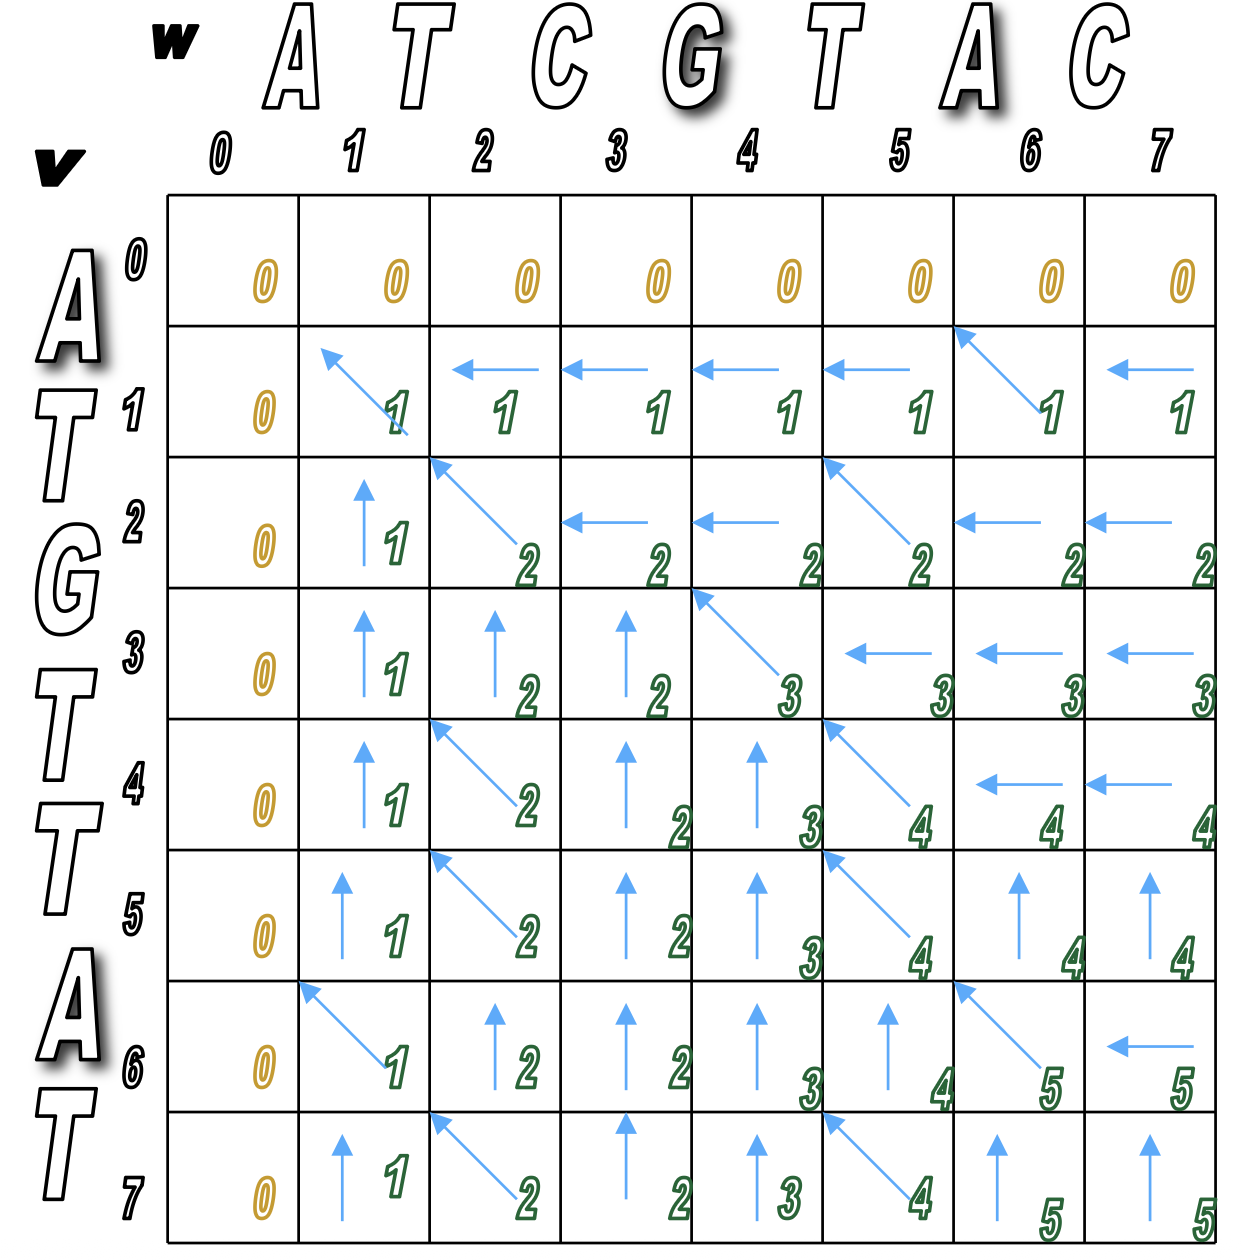
\includegraphics[width=0.7\textwidth]{images/backtracking.png}
    \caption{Didascalia dell'immagine}
    \label{fig:edit_grid complete}
\end{figure}
Per ricostruire una matrice di allineamento $A$ (di dimensione $2 \times k$, con $k \geq \max(n,m)$) che rifletta tale distanza, si utilizza la procedura di \textbf{backtracking} (percorso a ritroso) all'interno della griglia:

\begin{enumerate}
    \item Si parte dall'ultima cella, ovvero il nodo \textit{sink} $(n, m)$.
    \item Si risale la griglia all'indietro fino ad arrivare al nodo \textit{sorgente} $(0, 0)$. Ad ogni passo, ci si sposta verso la cella adiacente che ha fornito il valore minimo usato nell'equazione di ricorrenza (in caso di parità tra più direzioni ottime, se ne può scegliere una qualsiasi, ottenendo allineamenti alternativi ma con lo stesso score ottimale).
    \item Durante questa risalita, si costruisce la matrice di allineamento aggiungendo una colonna alla volta dall'ultima verso la prima:
    \begin{itemize}
        \item Se lo spostamento a ritroso è \textbf{diagonale} verso $(i-1, j-1)$, si aggiunge la colonna $\begin{pmatrix} v_i \\ w_j \end{pmatrix}$.
        \item Se lo spostamento a ritroso è \textbf{verticale} verso $(i-1, j)$, il carattere $v_i$ è allineato con un gap. Si aggiunge la colonna $\begin{pmatrix} v_i \\ \text{-} \end{pmatrix}$.
        \item Se lo spostamento a ritroso è \textbf{orizzontale} verso $(i, j-1)$, il carattere $w_j$ è allineato con un gap. Si aggiunge la colonna $\begin{pmatrix} \text{-} \\ w_j \end{pmatrix}$.
    \end{itemize}
    \item Il processo termina non appena si raggiunge la cella $(0, 0)$. 
\end{enumerate}

Le colonne così ottenute, lette nell'ordine inverso rispetto a come sono state ricostruite, formano la \textbf{matrice di allineamento globale}. Il \textbf{costo dell'allineamento} si calcola sommando il costo di ogni colonna della matrice:
\begin{equation}
    \text{costo}(A) = \sum_{\ell=1}^{k} \delta(A_{1,\ell}, A_{2,\ell})
\end{equation}
dove ogni colonna $\begin{pmatrix} A_{1,\ell} \\ A_{2,\ell} \end{pmatrix}$ può rappresentare un match, un mismatch oppure un indel. Quindi una colonna con due caratteri uguali ha costo $0$, mentre una colonna con due caratteri diversi oppure con un gap ha costo $1$. La somma dei costi di tutte le colonne coincide con il costo del cammino nella griglia e quindi con la distanza di edit $d_E(v,w)=S(n,m)$.
\newpage
\section{Come si modifica il metodo di cui sopra per calcolare la 
distanza di Hamming (se v e w hanno stessa lunghezza) e la 
longest common subsequence tra v e w}

Per adattare il metodo di calcolo della distanza di edit per ottenere la distanza 
di Hamming o Longest common subsequence (LCS), 
è necessario modificare le \textbf{operazioni consentite}, 
e di conseguenza la definizione della \textbf{funzione di costo} $\delta$ 
e l'algoritmo di \textbf{programmazione dinamica}.

\paragraph{Distanza di Hamming}

La \textbf{distanza di Hamming} si applica quando le due stringhe hanno la stessa 
lunghezza e si calcola confrontando i caratteri nelle stesse posizioni. 
Ogni posizione diversa contribuisce con costo $1$, mentre ogni posizione uguale 
contribuisce con costo $0$.

\begin{equation}
    d_H(v, w) = \text{numero di posizioni in cui } v \text{ e } w \text{ differiscono}
\end{equation}

\textbf{Esempio}

\begin{align*}
    S_1 &= ACCGT \\
    S_2 &= AGCGT
\end{align*}

Le due stringhe differiscono solo nella seconda posizione, dove $C \neq G$. Quindi:
\begin{equation}
    d_H(S_1,S_2)=1
\end{equation}

Se invece:
\begin{align*}
    S_1 &= ACCGT \\
    S_2 &= ACCGT
\end{align*}

non ci sono posizioni diverse, quindi:
\begin{equation}
    d_H(S_1,S_2)=0
\end{equation}

Per calcolare $d_H(v, w)$ utilizzando una griglia di edit definita per la distanza 
di edit, ma bisogna apportare alcune modifiche:
\begin{itemize}
    \item La griglia di edit sarà una matrice di dimensione $n \times m$ con $n = m$ (poiché le stringhe devono avere la stessa lunghezza).
    \item Gli archi consentiti saranno solo quelli diagonali, poiché non sono permesse operazioni di inserzione o delezione. 
    \item La funzione di costo $\delta$ sarà definita come:
    \begin{itemize}
        \item \textbf{match}: $\delta(v_i, w_j) = 0$ se $v_i = w_j$ 
        \item \textbf{mismatch}: $\delta(v_i, w_j) = 1$ se $v_i \neq w_j$
        \item \textbf{indel}: $\delta(v_i, w_j) = n (\infty)$ se $v_i$ o $w_j$ = \texttt{-} 
    \end{itemize}
\end{itemize}

Il \textbf{costo $n$} assegnato agli indel serve a penalizzare fortemente inserzioni e
delezioni. Infatti, poiché le due stringhe hanno la stessa lunghezza, il costo
massimo della distanza di Hamming è $n$, cioè il caso in cui tutti i caratteri
siano diversi. Se invece un allineamento usa un gap, per mantenere le due
sequenze della stessa lunghezza dovrà introdurre almeno due indel, con costo
totale almeno $2n$. Poiché $2n > n$, un allineamento con gap non potrà mai essere
ottimo. In questo modo l'algoritmo è forzato ad allineare solo caratteri in
\textbf{posizione corrispondente} (movimenti diagonali), e il costo finale coincide con il numero di mismatch.

Per calcolare il costo minimo si può usare ancora la programmazione dinamica,
come nel caso della distanza di edit. Indichiamo con $S(i,j)$ il costo minimo
per allineare il prefisso $v[1..i]$ con il prefisso $w[1..j]$.

I \textbf{casi base} diventano:
\begin{itemize}
    \item $S(0,0)=0$
    \item $S(i,0)=i \cdot n$ per $0 \leq i \leq n$
    \item $S(0,j)=j \cdot n$ per $0 \leq j \leq n$
\end{itemize}

Infatti, per allineare un prefisso non vuoto con una stringa vuota, è necessario
inserire solo gap, e ogni gap ha costo $n$.

Successivamente, si riempie il resto della griglia con la seguente
\textbf{equazione di ricorrenza}:
\begin{equation}
    S(i,j)=\min
    \begin{cases}
        S(i-1,j)+n & \text{(Delezione)} \\
        S(i,j-1)+n & \text{(Inserzione)} \\
        S(i-1,j-1)+\delta(v_i,w_j) & \text{(Match/Mismatch)}
    \end{cases}
\end{equation}

dove:

\begin{equation}
    \delta(v_i,w_j)=
    \begin{cases}
        0 & \text{se } v_i=w_j \\
        1 & \text{se } v_i \neq w_j
    \end{cases}
\end{equation}

Il valore nel nodo finale:
\begin{equation}
    S(n,n)
\end{equation}

coincide quindi con la distanza di Hamming:

\begin{equation}
     S(n,n)=d_H(v,w)
\end{equation}

La \textbf{matrice di allineamento} che si ottiene non contiene gap, ma solo colonne del tipo:

\[
\begin{pmatrix}
v_i \\
w_i
\end{pmatrix}
\]

per ogni posizione $i$. Ogni colonna ha costo $0$ se i due simboli sono uguali e
costo $1$ se sono diversi. La somma dei costi delle colonne è quindi esattamente
il numero di mismatch tra $v$ e $w$.
In questo modo, la distanza di Hamming può essere vista come un caso particolare
della distanza di edit in cui inserzioni e delezioni sono rese non convenienti
tramite un costo molto alto.

\paragraph{Longest Common Subsequence (LCS)}
Date due sequenze $v = v_1 v_2 \ldots v_n$ e $w = w_1 w_2 \ldots w_m$ 
la \textbf{longest common subsequence (LCS)} di $v$ e $w$ è la sequenza di posizioni
$1 \leq i_1 < i_2 < \ldots < i_k \leq n$ e $1 \leq j_1 < j_2 < \ldots < j_k \leq m$
tale che la $i$-esima posizione di $v$ e la $j$-esima posizione di $w$ contengono lo stesso simbolo, 
ovvero $v_{i_t} = w_{j_t}$ per ogni $t = 1, 2, \ldots, k$. 
La lunghezza della longest common subsequence è indicata con $LCS(v,w)$.

\textbf{Esempio}

Consideriamo:
\begin{align*}
    v &= ATCTGATC \\
    w &= TGCATAC
\end{align*}

Un possibile allineamento tra $v$ e $w$ è:
\[
A =
\begin{pmatrix}
A & \textcolor{red}{T} & \text{-} & \textcolor{red}{C} & \text{-} & \textcolor{red}{T} & G & \textcolor{red}{A} & T & \textcolor{red}{C} \\
\text{-} & \textcolor{red}{T} & G & \textcolor{red}{C} & A & \textcolor{red}{T} & \text{-} & \textcolor{red}{A} & \text{-} & \textcolor{red}{C}
\end{pmatrix}
\]

Le colonne evidenziate in rosso sono i \textbf{match}, cioè le colonne in cui i due
simboli allineati sono uguali. Il cammino corrispondente nella griglia è:
\[
\begin{aligned}
(0,0) &\rightarrow (1,0) \rightarrow \textcolor{red}{(2,1)}
\rightarrow (2,2) \rightarrow \textcolor{red}{(3,3)} \rightarrow (3,4) \\
&\rightarrow \textcolor{red}{(4,5)} \rightarrow (5,5)
\rightarrow \textcolor{red}{(6,6)} \rightarrow (7,6)
\rightarrow \textcolor{red}{(8,7)}
\end{aligned}
\]

Quindi le posizioni scelte in $v$ sono:
\[
    2 < 3 < 4 < 6 < 8
\]

e le posizioni corrispondenti in $w$ sono:
\[
    1 < 3 < 5 < 6 < 7
\]

La \textbf{sottosequenza comune} letta nelle colonne di match è:
\[
    TCTAC
\]

In questo esempio la lunghezza della longest common subsequence è quindi:
\[
    LCS(v,w)=5
\]

Anche per LCS è possibile utilizzare una \textbf{griglia di edit} di dimensione $(n+1) \times (m+1)$, con $n = |v|$ e $m = |w|$, con archi pesati e applicare la \textbf{programmazione dinamica}.
Tuttavia, come per la distanza di Hamming, è necessario modificare operazioni
consentite, funzione di costo $\delta$ e algoritmo di programmazione dinamica. 
In particolare dovendo trovare le posizioni dove $v$ e $w$ hanno simboli uguali,
andrà considerato il \textbf{movimento diagonale}, solo in caso di match.
Inoltre al contrario di edit e hamming serve trovare la più lunga sottosequenza comune,
quindi servirà modificare i valori di costo per riflettere questa differenza.
andando ad escludere i mismatch dall'allineamento.

Quindi la \textbf{funzione di costo} $\delta$ sarà definita come:
\begin{itemize}
    \item \textbf{match}: $\delta(v_i, w_j) = 1$ se $v_i = w_j$ (l'arco diagonale da $(i-1,j-1)$ a $(i,j)$)
    \item \textbf{Indel} (inserzione o delezione): $\delta(v_i,\text{-})=0$ per una delezione (l'arco verticale da $(i-1,j)$ a $(i,j)$) e $\delta(\text{-},w_j)=0$ per una inserzione (l'arco orizzontale da $(i,j-1)$ a $(i,j)$).
\end{itemize}

Per calcolare la LCS fra due sequenze si utilizza la programmazione dinamica ma cambia l'obbiettivo: invece di minimizzare il costo, si massimizza il numero di match.
non cerca più di minimizzare il costo totale, ma di massimizzare il numero di match (lunghezza della sottosequenza comune).+

Indichiamo con $S(i,j)$ la lunghezza della LCS tra il prefisso $v[1..i]$ e il prefisso $w[1..j]$.

I \textbf{casi base} diventano:
\begin{itemize}
    \item $S(0,0)=0$
    \item $S(i,0)=0$ per $0 \leq i \leq n$
    \item $S(0,j)=0$ per $0 \leq j \leq m$
\end{itemize}

Infatti, se una delle due sequenze è vuota, non esiste alcuna sottosequenza comune non vuota, quindi la lunghezza della LCS è $0$.

Si riempie il resto della griglia con la seguente \textbf{equazione di ricorrenza}:
\begin{equation}
    S(i,j)=\max
    \begin{cases}
        S(i-1,j) & \text{(salto } v_i\text{)} \\
        S(i,j-1) & \text{(salto } w_j\text{)} \\
        S(i-1,j-1)+1 & \text{se } v_i=w_j
    \end{cases}
\end{equation}

Il valore nel nodo finale:
\begin{equation}
    S(n,n)
\end{equation}

coincide quindi con la lunghezza della longest common subsequence:

\begin{equation}
     S(n,m)=LCS(v,w)
\end{equation}

Effettuando il \textbf{backtracking} nella griglia, partendo dal nodo finale
$(n,m)$ e risalendo fino al nodo sorgente $(0,0)$, è possibile ricostruire
una matrice di allineamento $A$.

Per ottenere la \textbf{longest common subsequence}, si considerano solo le
colonne di $A$ che corrispondono a un match, cioè colonne del tipo:

\[
\begin{pmatrix}
v_i \\
w_j
\end{pmatrix}
\]

con $v_i = w_j$.

I simboli letti in queste colonne, nell'ordine dell'allineamento, formano la
longest common subsequence.

\newpage
\section{In che cosa differisce l’allineamento globale dal locale e dal semi-globale anche in termini
di calcolo dello stesso}

Siano $V = v_1 v_2 \ldots v_n$ e $W = w_1 w_2 \ldots w_m$ due stringhe di lunghezza $n$ e $m$ definite su un alfabeto $\Sigma$. Si indica con $-$ il simbolo di gap
e con $\delta : (\Sigma \cup \{-\}) \times (\Sigma \cup \{-\}) \rightarrow \mathbb{N}$ una funzione di costo che assegna un costo a ogni coppia di simboli (compresi i gap), in particolare:
\begin{itemize}
    \item $\delta(v_i,w_j)=k$ se $v_i=w_j$ (match)
    \item $\delta(v_i,w_j)=s$ se $v_i \neq w_j$ (mismatch)
    \item $\delta(v_i,-)=\delta(-,w_j)=d$
\end{itemize}

Un allineamento tra $V$ e $W$ è una matrice $A$ di dimensione $2 \times k$ (con $k \geq \max(n,m)$) 
ottenuta inserendo eventualmente i gap nelle sequenza,
in modo tale che, eliminando i gap dalla prima riga, si ottiene $V$,
ed eliminando i gap dalla seconda riga, si ottiene $W$.
Ogni colonna di $A$ rappresenta un un match, mismatch, inserzione o delezione.
Il punteggio di allineamento è dato dalla somme dei punteggi delle singole colonne
\begin{equation}
    \text{C}(A) = \sum_{i=1}^{k} \delta(A_{1,i}, A_{2,i})
\end{equation}

Per calcolare un allineamento ottimo si usa una griglia di edit di dimensione
$(n+1) \times (m+1)$, in cui $C(i,j)$ rappresenta lo score ottimo per allineare il prefisso $v[1..i]$ con il prefisso $w[1..j]$.

\paragraph{Allineamento Globale}

L'\textbf{allineamento globale} di due sequenze $V$ e $W$ è un allineamento che considera entrambe le sequenze nella loro interezza.
Quindi l'obbiettivo è trovare la matrice di allineamento $A$ di score ottimo
tra tutta la sequenza $V$ e tutta la sequenza $W$.

Nel calcolo tramite programmazione dinamica, $S(i,j)$ rappresenta lo score
ottimo di allineamento globale fra il prefisso $V_i$ e il prefisso $W_j$.

I \textbf{casi base} sono:
\begin{itemize}
    \item $S(0,0)=0$
    \item $S(i,0)= i \cdot d$
    \item $S(0,j)= j \cdot d$
\end{itemize}

Dove $d$ è il costo dell'inserimento di un gap. Infatti, per allineare un prefisso non vuoto con una stringa vuota, è necessario inserire solo gap, e ogni gap ha costo $d$.

per $i > 0$ e $j > 0$ la ricorrenza è:
\begin{equation}
    S(i,j) = \min (\max)
    \begin{cases}
        S(i-1,j-1) + \delta(v_i,w_j) & \text{(match/mismatch)} \\
        S(i-1,j) + \delta(v_i,-) & \text{(delezione)} \\
        S(i,j-1) + \delta(-,w_j) & \text{(inserzione)}
    \end{cases}
\end{equation}

Poichè si considerano entrambe le sequenze nella loro interezza, il punteggio ottimo si trova nel nodo finale $S(n,m)$.

La ricostruzione dell'allineamento avviene tramite backtracking, partendo da $S(n,m)$ e risalendo fino a $S(0,0)$, seguendo i movimenti che hanno portato al punteggio ottimo.
Si ottiene così la matrice di allineamento $A$.

\paragraph{Allineamento Locale}

Date due stringe:
\[
V = v_1 v_2 \ldots v_{i-1} v_1 v_{i+1} \ldots v_n \quad \text{e} \quad W = w_1 w_2 \ldots w_{j-1} w_j w_{j+1} \ldots w_m
\]
un \textbf{allineamento locale} consiste nel determinare il miglior allineamento globale
tra una sottostringa di $V$ e una sottostringa di $W$.

Quindi, a differenza dell'allineamento globale, non si vuole necessariamente
allineare tutta la sequenza $V$ con tutta la sequenza $W$, ma si vogliono
individua le regioni più simili contenute nelle sequenze.

Formalmente, l'obbiettivo è quindi di trovare due sotto stringe $V' = v_i v_{i+1} \ldots v_{i+k}$ e $W' = w_j w_{j+1} \ldots w_{j+k}$ (con $k \geq 0$) tali che lo score di 
allineamento globale fra le due sottostringhe sia massimi fra tutte le possibile coppie di sottostringhe in $V$ e $W$.
\\
\\
Anche per l'allineamento locale si utilizza la griglia di edit $S$ di dimensione: $(n+1) \times (m+1)$,
dove però $S(i,j)$ rappresenterà il miglior score di allinaemento globale
tra due sottostringhe che terminano rispettivamente in $v_i$ e $w_j$.
\\
\\
In altre parole, $S(i,j)$ non rappresenta lo score tra prefissi di $V$ e $W$,
ma il miglior score tra tutte le coppie di sottostringhe che terminano in $v_i$ e $w_j$.
Lo scor dell'allineamento locale tra $V$ e $W$ sarà quindi il massimo valore
presente nella matrice $S$.

I \textbf{casi base} sono:
\begin{itemize}
    \item $S(0,0)=0$
    \item $S(i,0)=0$ per $0 \leq i \leq n$
    \item $S(0,j)=0$ per $0 \leq j \leq m$
\end{itemize}

A differenza dell'allineamento globale, qui non si inizializza la prima riga
e la prima colonna con il costo dei gap, in quanto le parti iniziali delle sequenze
che non appartengono alla sottostringa ottima posso essere ignorate. L'allineamento, infatti,
può inzizare in qualunque punto della matrice.

Per $i > 0$ e $j > 0$ la ricorrenza è:
\begin{equation}
    S(i,j) = \max (\min) \begin{cases}
        0 \\
        S(i-1,j-1) + \delta(v_i,w_j)\\
        S(i-1,j) + \delta(v_i,-) \\
        S(i,j-1) + \delta(-,w_j)
    \end{cases}
\end{equation}

Il primo caso, con punteggio $0$, è la differenza principale rispetto
all'allineamento globale. Infatti, se tutte le opzioni di allineamento hanno un punteggio negativo, è preferibile non allineare nulla
quindi interrompere l'allineamento corrente e iniziare un novo allineamento a partire dalla cella successiva. 
\\
Una volta riempita la matrice $S$, lo score ottimo dell'allineamento locale non si trova necessariamente in $S(n,m)$ ma è:
\[
    \max_{0 \leq i \leq n, 0 \leq j \leq m} S(i,j)
\]
cioè il massimo valore presente nella matrice.
\begin{figure}[h]
    \centering
    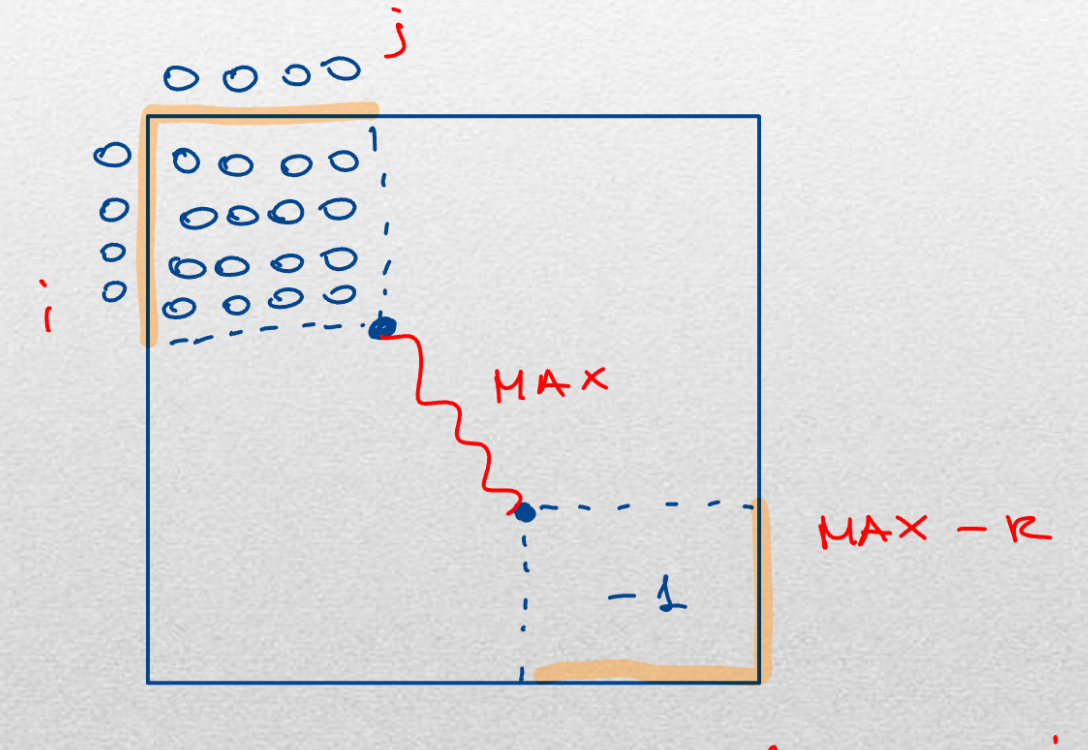
\includegraphics[width=0.7\textwidth]{images/local_allignment.png}
    \caption{Didascalia dell'immagine}
    \label{fig:local_allignment}
\end{figure}

La ricostruzione dell'allineamento avviene tramite backtracking, partendo dalla cella che contiene il punteggio massimo.
Il backtracking procede a ritroso seguendo i movimenti che hanno portato al punteggio ottimo e si ferma quando raggiunge una cella con punteggio $0$, che rappresenta
l'inizio dell'allineamento locale ottimo.

\begin{figure}[h]
    \centering
    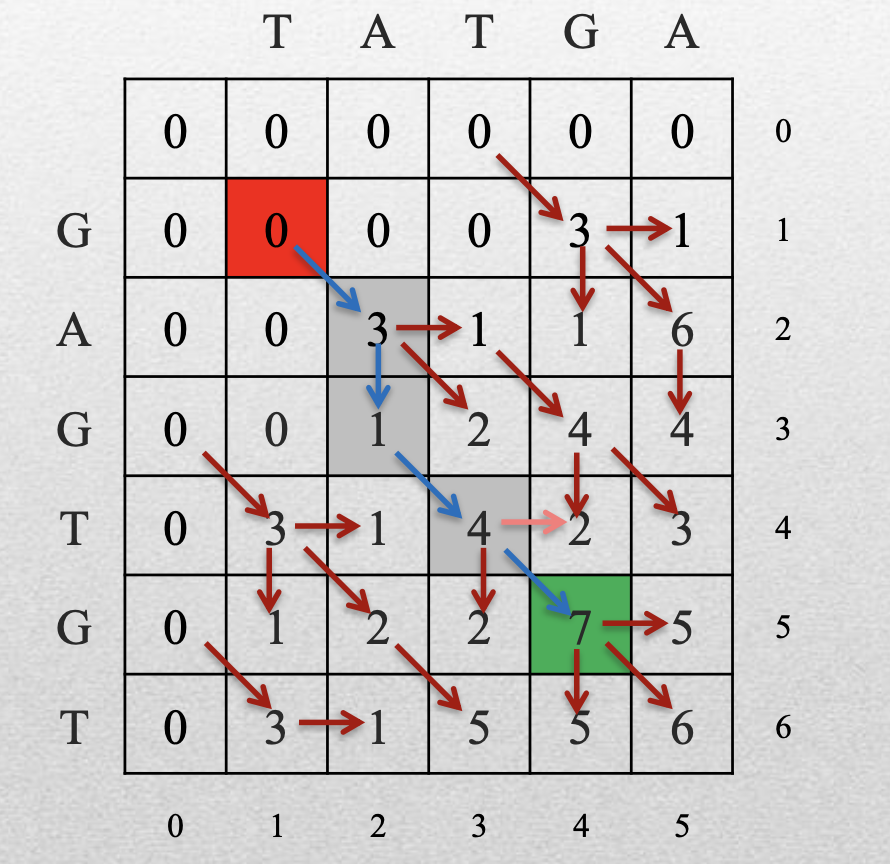
\includegraphics[width=0.7\textwidth]{images/back_locale.png}
    \caption{Didascalia dell'immagine}
    \label{fig:back_locale}
\end{figure}

\paragraph{Allineamento Semi-globale}

L'\textbf{allineamento semi-globale} di due sequenze
$V=v_1v_2\dots v_m$ e $W=w_1w_2\dots w_n$ è una famiglia di problemi di
allineamento in cui non si richiede necessariamente di allineare entrambe le
sequenze per intero, come nell'allineamento globale, ma non si cercano nemmeno
due sottostringhe completamente arbitrarie, come nell'allineamento locale.

L'idea generale è cercare un allineamento globale ottimo tra due porzioni
vincolate delle sequenze. Questo significa che il problema specifica che tipo
di porzione si può scegliere: un prefisso, un suffisso, una sottostringa,
oppure l'intera sequenza. Una volta scelta tale porzione, essa viene allineata
globalmente con l'altra porzione.

Quindi, in generale, l'allineamento semi-globale cerca un allineamento globale
ottimo tra $V[a..b]$ e $W[c..d]$,
dove però gli indici $a,b,c,d$ non sono completamente liberi come nel locale,
ma sono vincolati dal tipo di problema, in particolare:
\begin{itemize}
    \item se si cerca un prefisso di $V$, allora la porzione deve iniziare da
    $v_1$, quindi è del tipo $V[1..b]$;
    \item se si cerca un suffisso di $W$, allora la porzione deve terminare in
    $w_n$, quindi è del tipo $W[c..n]$;
    \item se si cerca una sottostringa di $V$, allora la porzione può iniziare
    e finire in posizioni interne, quindi è del tipo $V[a..b]$;
    \item se si considera tutta $W$, allora la porzione è fissata ed è
    $W[1..n]$.
\end{itemize}

La stessa cosa vale per la sequenza $W$.

Dal punto di vista del calcolo, anche l'allineamento semi-globale usa una
matrice dinamica $S$ di dimensione:
\[
    (m+1) \times (n+1)
\]

La ricorrenza interna è in genere la stessa dell'allineamento globale:
\[
    S(i,j)=\max
    \begin{cases}
        S(i-1,j-1)+\delta(v_i,w_j)\\
        S(i-1,j)+\delta(v_i,-)\\
        S(i,j-1)+\delta(-,w_j)
    \end{cases}
\]

La differenza rispetto al globale sta nel fatto che non sempre l'ottimo viene
cercato nella cella finale $S(m,n)$. A seconda del tipo di porzione considerata,
lo score ottimo può essere cercato nell'ultima riga, nell'ultima colonna, in
tutta la matrice o in un'altra regione specifica.

Anche l'\textbf{inizializzazione} e il \textbf{punto di arresto del backtracking}
dipendono dal problema semi-globale considerato: le parti della sequenza che
possono essere ignorate non vengono penalizzate, mentre le parti che devono
essere effettivamente allineate vengono trattate come in un allineamento
globale.

\textbf{1. Prefisso di $V$ contro tutta $W$}

\[
    V[1..r] \quad \text{contro} \quad W[1..m]
\]

Lo score ottimo si cerca nell'ultima colonna:
\[
    \max_{0 \leq i \leq n} S(i,m)
\]
perché $W$ deve essere considerata interamente, mentre il prefisso di $V$ può
terminare in una qualunque posizione $i$.

\begin{figure}[H]
    \centering
    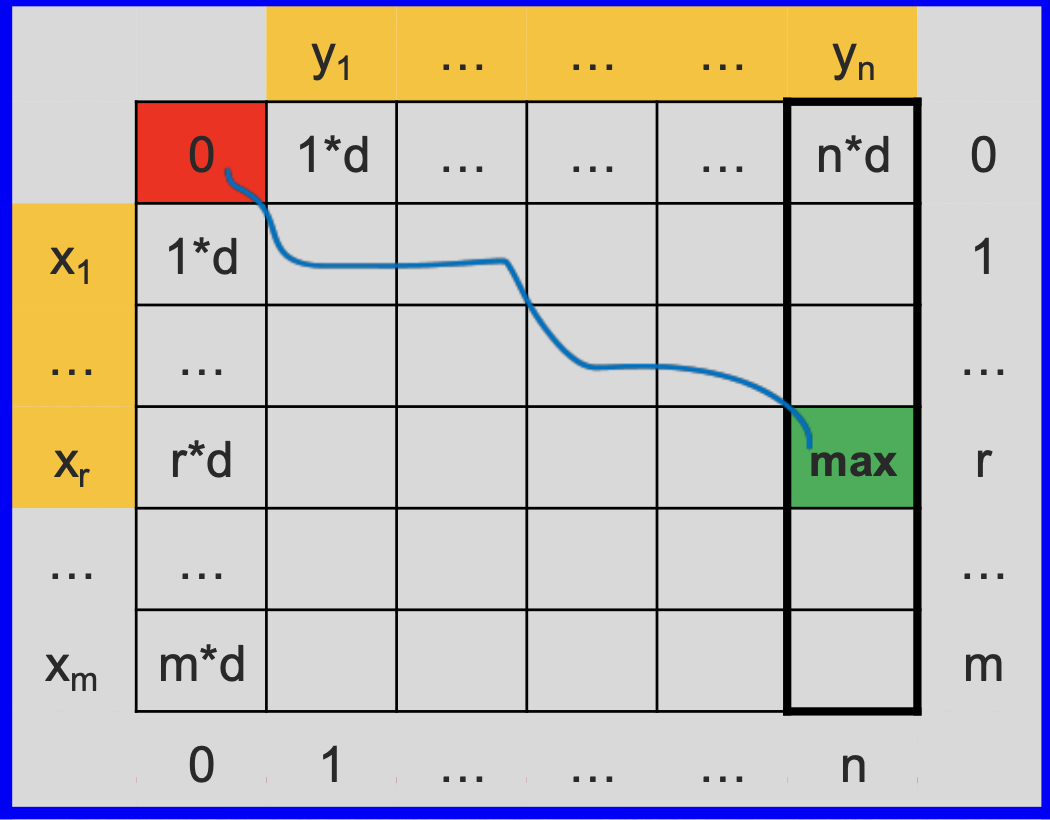
\includegraphics[width=0.6\textwidth]{images/preXvsY.png}
    \caption{Allineamento tra un prefisso di $V$ e tutta $W$.}
    \label{fig:semiglobale-prefisso-v-tutta-w}
\end{figure}

\textbf{2. Tutta $V$ contro prefisso di $W$}

\[
    V[1..n] \quad \text{contro} \quad W[1..c]
\]

Lo score ottimo si cerca nell'ultima riga:
\[
    \max_{0 \leq j \leq m} S(n,j)
\]
perché $V$ deve essere considerata interamente, mentre il prefisso di $W$ può
terminare in una qualunque posizione $j$.

\begin{figure}[H]
    \centering
    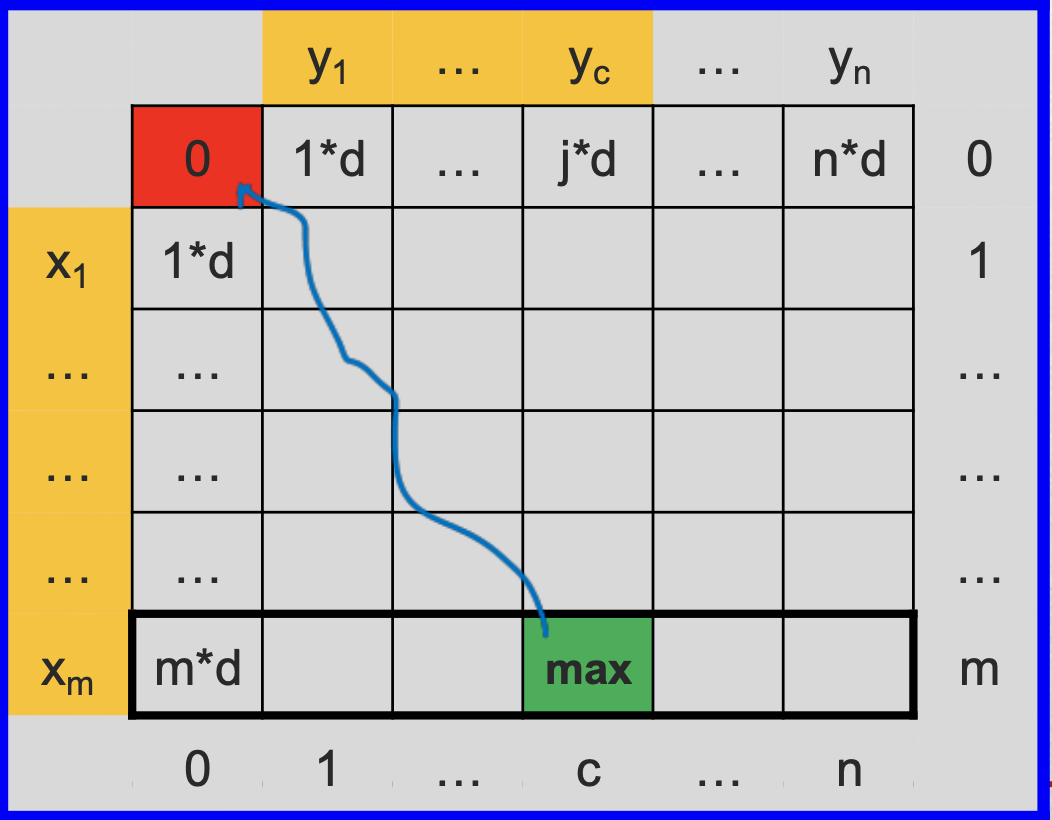
\includegraphics[width=0.6\textwidth]{images/XvsPreY.png}
    \caption{Allineamento tra tutta $V$ e un prefisso di $W$.}
    \label{fig:semiglobale-tutta-v-prefisso-w}
\end{figure}

\textbf{3. Prefisso di $V$ contro prefisso di $W$}

\[
    V[1..r] \quad \text{contro} \quad W[1..c]
\]

Lo score ottimo si cerca in tutta la matrice:
\[
    \max_{0 \leq i \leq n,\ 0 \leq j \leq m} S(i,j)
\]
perché entrambi i prefissi possono terminare in posizioni non fissate.

\begin{figure}[H]
    \centering
    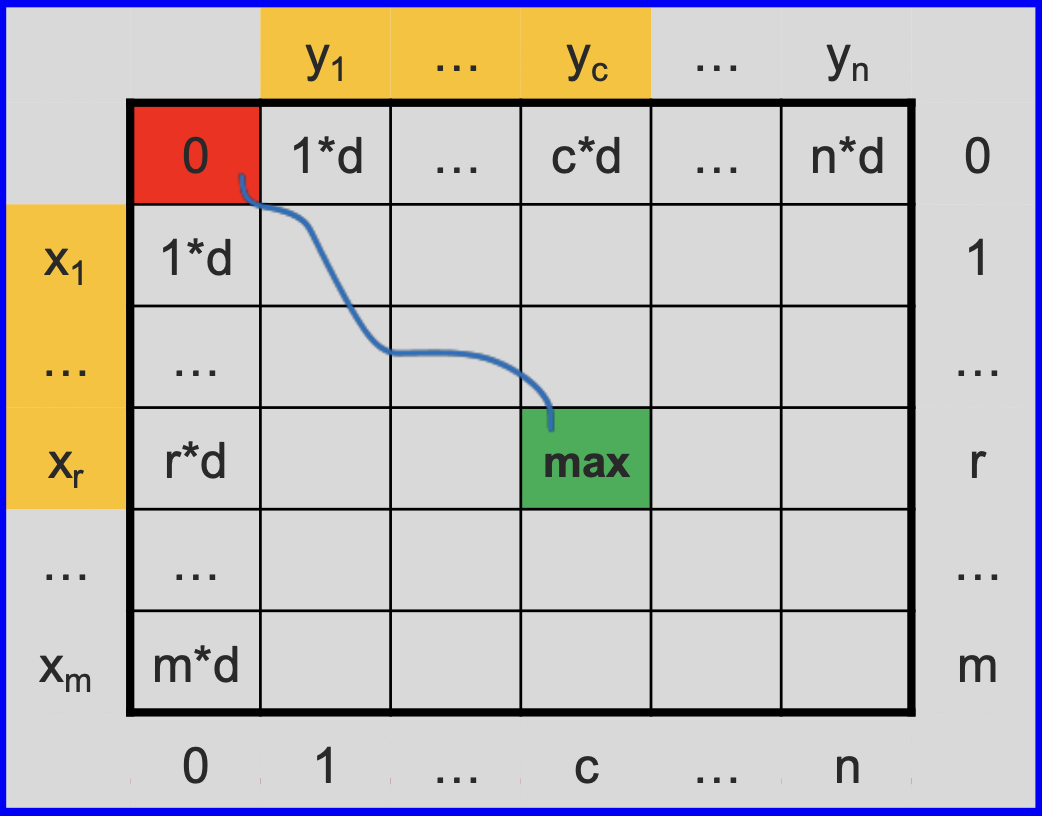
\includegraphics[width=0.6\textwidth]{images/preXvsPreY.png}
    \caption{Allineamento tra un prefisso di $V$ e un prefisso di $W$.}
    \label{fig:semiglobale-prefisso-v-prefisso-w}
\end{figure}

\textbf{4. Suffisso di $V$ contro suffisso di $W$}

\[
    V[a..n] \quad \text{contro} \quad W[c..m]
\]

Lo score ottimo si trova in:
\[
    S(n,m)
\]
perché entrambi i suffissi devono terminare alla fine delle rispettive sequenze.
Le parti iniziali non appartenenti ai suffissi possono invece essere ignorate.

\begin{figure}[H]
    \centering
    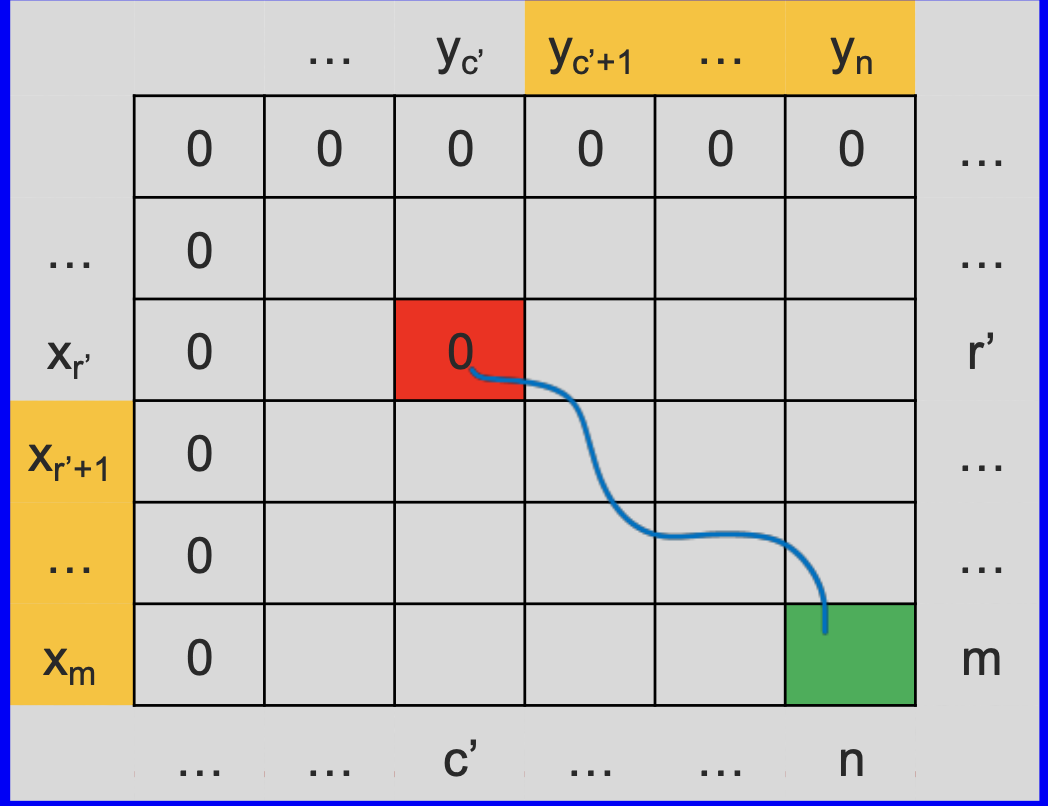
\includegraphics[width=0.6\textwidth]{images/suffXvsSuffY.png}
    \caption{Allineamento tra un suffisso di $V$ e un suffisso di $W$.}
    \label{fig:semiglobale-suffisso-v-suffisso-w}
\end{figure}

\textbf{5. Suffisso di $V$ contro prefisso di $W$}

\[
    V[a..n] \quad \text{contro} \quad W[1..c]
\]

Lo score ottimo si cerca nell'ultima riga:
\[
    \max_{0 \leq j \leq m} S(n,j)
\]
perché il suffisso di $V$ deve terminare in $v_n$, mentre il prefisso di $W$ può
terminare in una qualunque posizione $j$.

\begin{figure}[H]
    \centering
    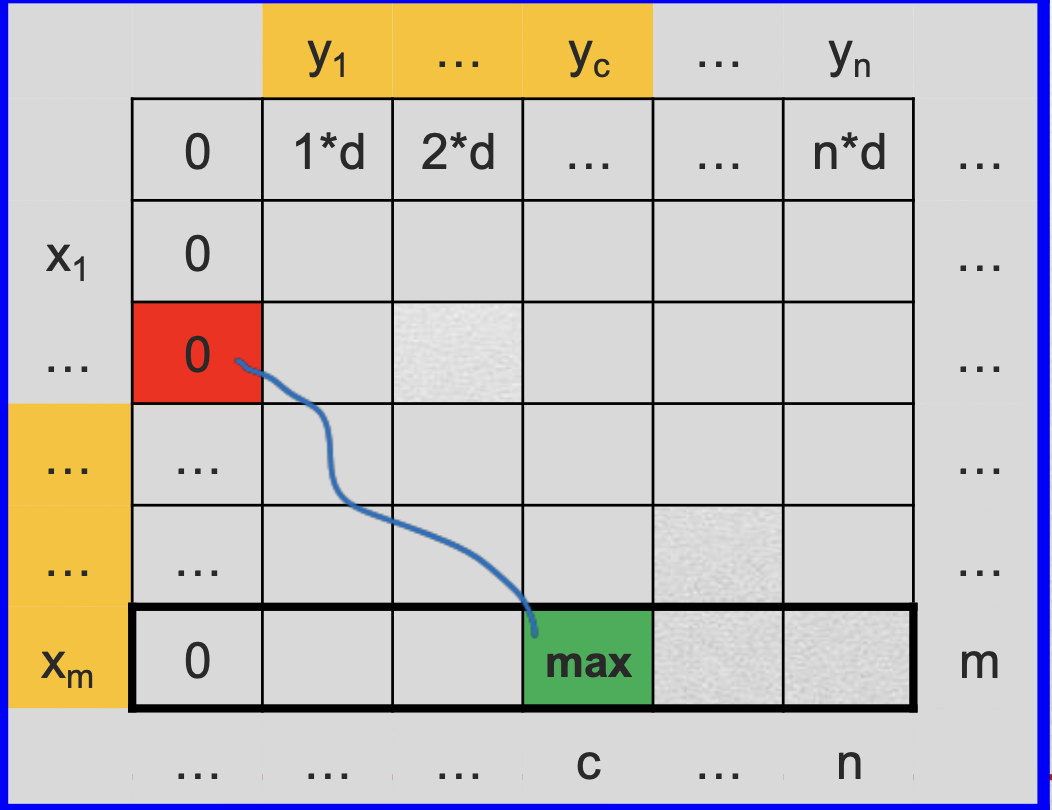
\includegraphics[width=0.6\textwidth]{images/SufPre.png}
    \caption{Allineamento tra un suffisso di $V$ e un prefisso di $W$.}
    \label{fig:semiglobale-suffisso-v-prefisso-w}
\end{figure}

\textbf{6. Sottostringa di $V$ contro tutta $W$}

\[
    V[a..b] \quad \text{contro} \quad W[1..m]
\]

Lo score ottimo si cerca nell'ultima colonna:
\[
    \max_{0 \leq i \leq n} S(i,m)
\]
perché $W$ deve essere usata tutta, mentre la sottostringa di $V$ può terminare
in una qualunque posizione $i$.

\begin{figure}[H]
    \centering
    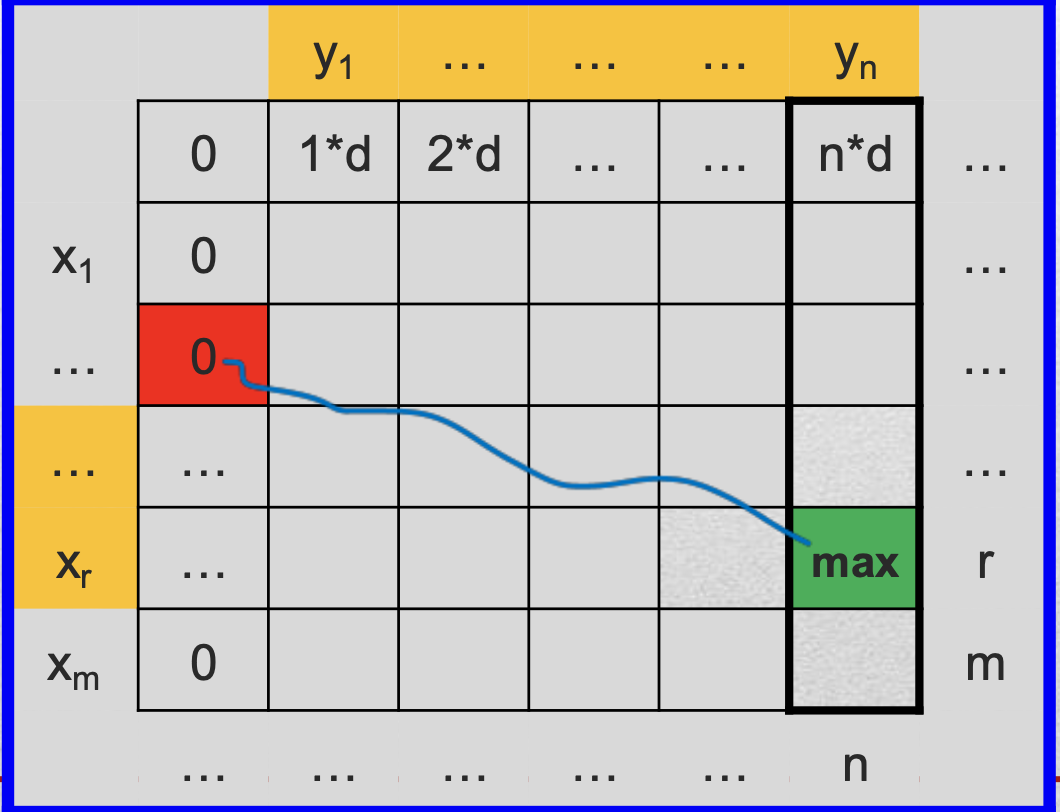
\includegraphics[width=0.6\textwidth]{images/subvsfull.png}
    \caption{Allineamento tra una sottostringa di $V$ e tutta $W$.}
    \label{fig:semiglobale-sottostringa-v-tutta-w}
\end{figure}



\end{document}
